\section{Proposed Method}
\label{sec:method}

A complete pipeline of Shape-Constrained Neural Network (SCNN) is illustrated in Figure~\ref{FigSCNN}.
The framework is trained end-to-end and consists of three key components:
1) a multi-task neural network based on FCN,
2) proposed joint max pooling and
3) local optimizing strategy to fuse the multi-outputs into final segmentation mask.
%
\begin{figure*}
    \begin{center}
        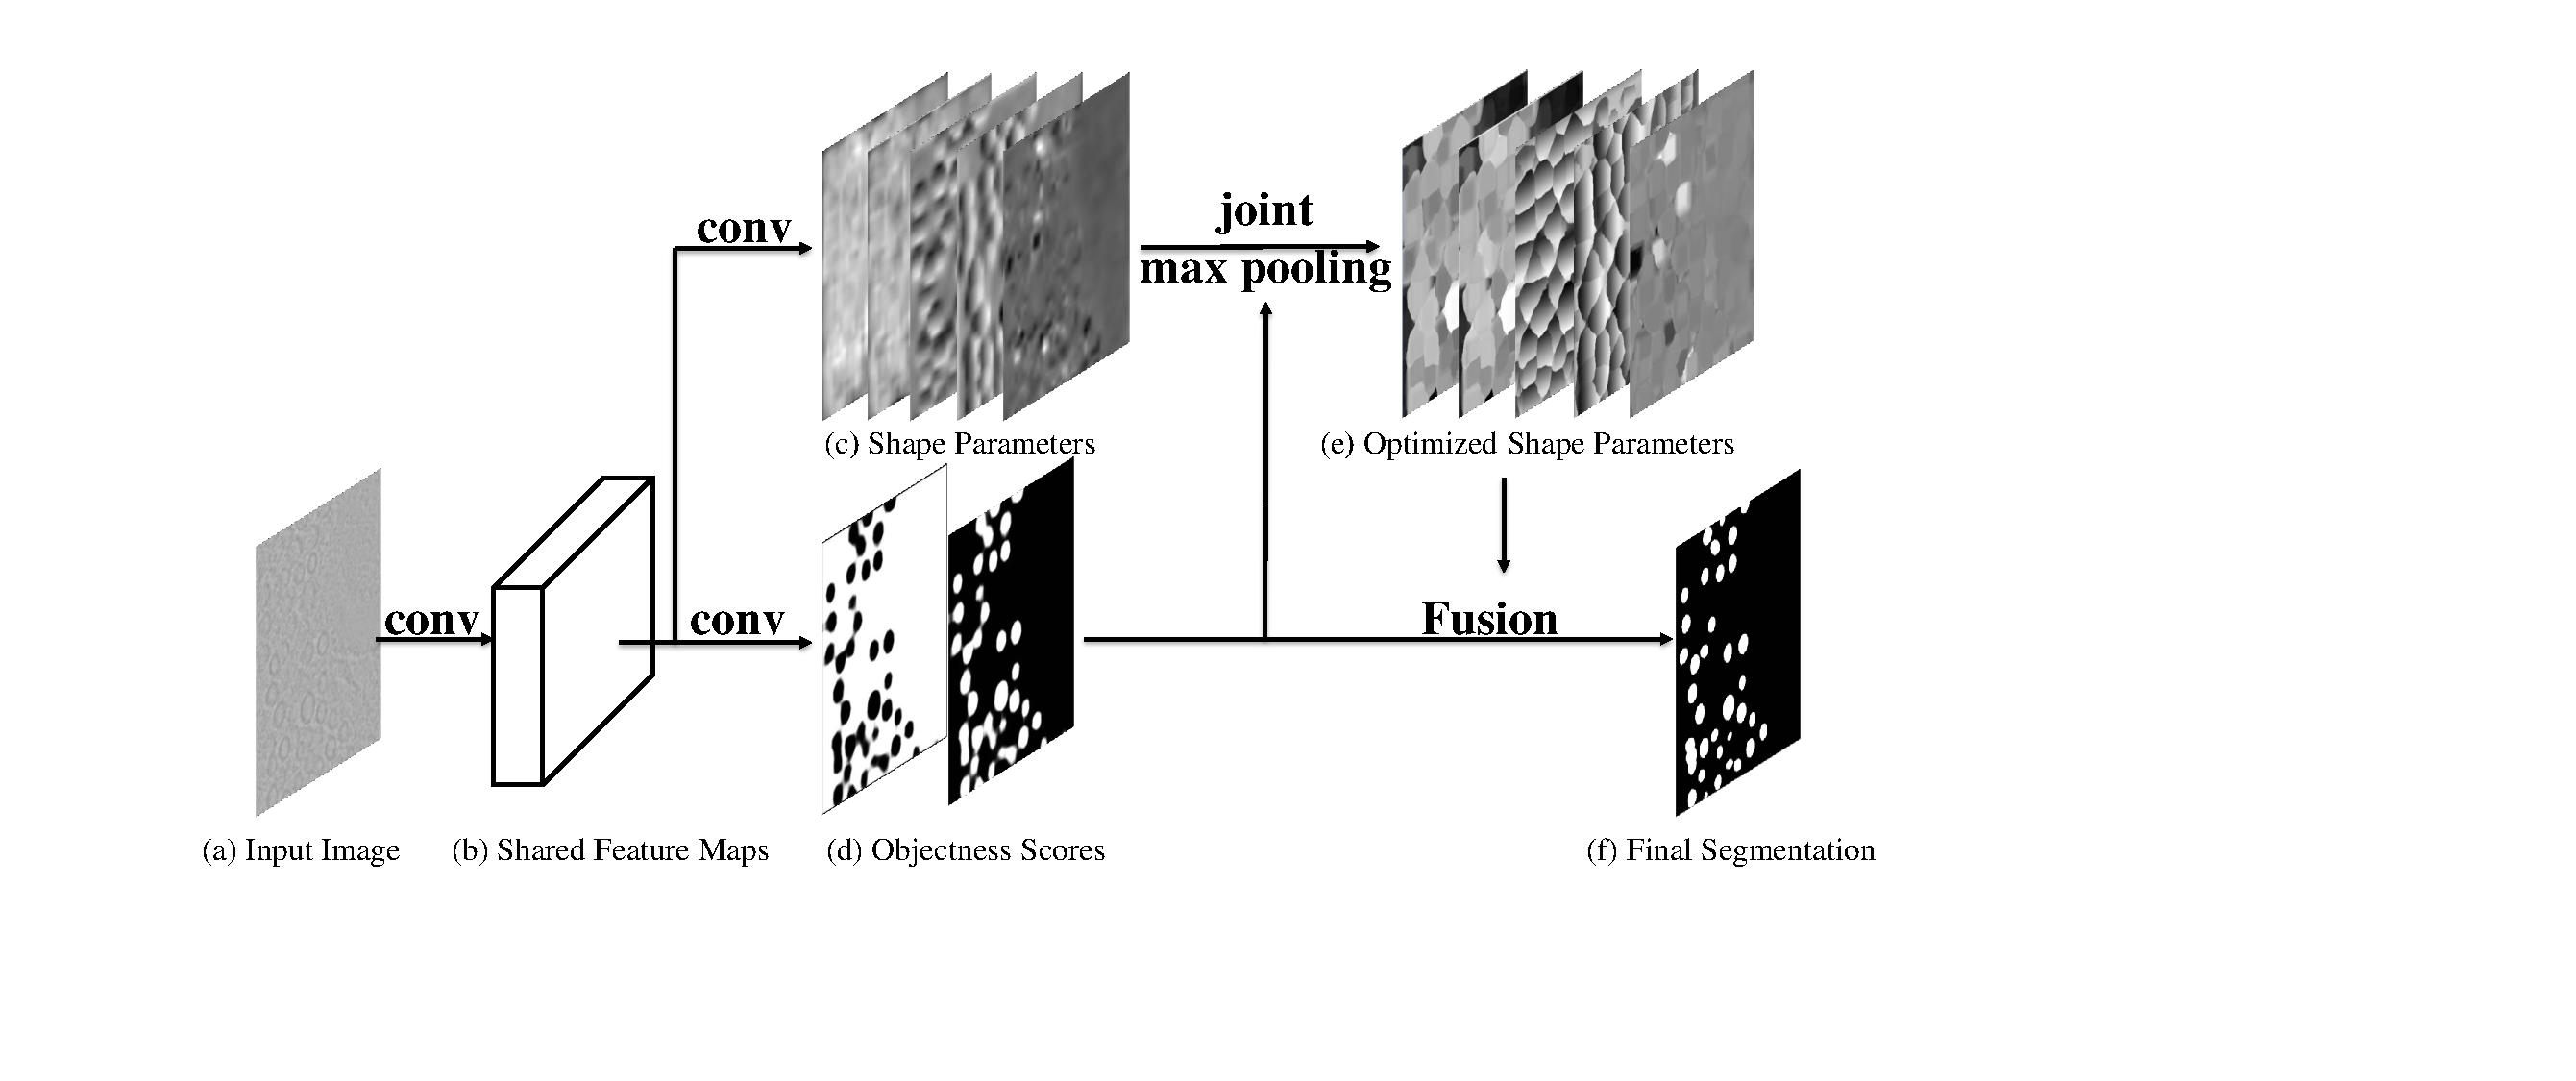
\includegraphics[width=6.8in]{figures/FigSCNN.pdf}
    \end{center}
    \caption{Overview of our proposed scnet. Given an image (a), multi-task neural network simultaneously predict objectness scores (d) and shape parameters of objects (d) using shared feature maps (b).
    Then a joint max pooling is applied to pool (c) with (d) and output new shape parameters (e).
    Finally, segmentation mask (f) is obtained by fusing objectness (d) with the parameterized contour description (e).}
    \label{FigSCNN}
\end{figure*}

Given an input image, the first part is a multi-task FCN which separately predicts objectness scores and shape parameters maps (Sec.~\ref{sec:multi-task-fcn}).
Then two branches integrate with each other by a joint max pooling layer (Sec.~\ref{sec:joint-max-pooling}) and a local fusion step to finally predict the shape-constrained segmentation (Sec.~\ref{sec:fusion}).

\subsection{Multi-task FCN}
\label{sec:multi-task-fcn}

The architecture of our multi-task learning network is shown in Figure~\ref{FigMTN}.
It simultaneously predicts an objectness map $p$ and an auxiliary map $t$ as complementary information.
The feature extracting part is shared and based on the publicly available DeepLab model~\cite{Chen2014a}, which introduces zeros into the filters to enlarge its Field-of-View.
Subsequently, extracted feature maps of last shared convolution layer are fed into two individual branches.
In each branch, successive two convolution layers, respectively with kernel size of $3\times3$ and $1\times1$, are applied to shared feature map, and then an upsampling layer restores their resolution to the input image size.
During training, the parameters of shared layers are jointly optimized, while the parameters of two branches are updated separately.

Instead of directly predicting contour probabilities like \cite{Chen2016a,Xu2016}, we choose the parameterized expression of objects shape as our complementary information, which emphasizes more on the overall shape of an object.
For example in our task for vesicle segmentation, the ellipse shape is applied as our prior shape knowledge and formulated by $5$ parameters: $\{\theta, \mu_c, \nu_c, a, b\}$.
$\theta$ is the rotated angle of the major axis from $x-$axis.
$(\mu_c, \nu_c)$ are the coordinates of elliptical center.
And $a$, $b$ are respectively the lengths of the major and minor axis.
With this definition, our auxiliary map $p$ has $5$ channels, each of which corresponds to one parameter.
For better regression, we further normalize the shape parameters by image width and height so that they fall in $[0,1]$:
\begin{eqnarray}\label{EqMax}
\begin{aligned}
p_i= \{\theta,\frac{\mu-\mu_c}{w},\frac{\nu-\nu_c}{h},\frac{a}{w},\frac{b}{h}\}
\end{aligned}
\end{eqnarray}
where $p_i$ is a vector regressed on position $i$, consisting of shape parameters of a nearest object.
$(\mu, \nu)$ are spatial coordinates of $p_i$.
and $w$,$h$ are image width and height.

The objective function follows the multi-task loss in~\cite{Ren2015}.
Our loss of multi-task FCN for an image is defined by:
\begin{eqnarray}\label{EqLoss}
\begin{aligned}
L(p,t) &= \frac{1}{N}(\sum_{i}L_{cls}(p_i,p^*_{i})+\lambda\sum_{i}p^*_{i}L_{reg}(t_{i},t^*_{i}))
\end{aligned}
\end{eqnarray}
where $N$ is the pixel number of input image.
$p^*_i$ and $t^*_i$ are the ground truth of objectness score and shape parameters.
The classification loss $L_{cls}$ is a soft-max loss over different classes.
And the regression loss $L_{reg}$ is the smooth $L_1$ loss in \cite{Ren2015} defined by
\begin{eqnarray}
\label{EqSmoothL1}
\begin{aligned}
L_{reg}(t_i,t^*_{i}) =\left\{\begin{array}{cc}
|t_i-t^*_{i}|&if~|t_{i}-t^*_{i}|>1\\
\frac{1}{2}(t_{i}-t^*_{i})^2&else\\
\end{array}\right.
\end{aligned}
\end{eqnarray}

Especially, we only consider the regression loss with positive $p^*_i$ in Eq.~\ref{EqLoss}, because most predicted $t_i$ with negative $p^*_i$ will be abandoned in next section by proposed joint max pooling.
And $\lambda$ is a balancing weight between $L_{cls}$ and $L_{reg}$.

\subsection{Joint Max Pooling}
\label{sec:joint-max-pooling}

Obtained from two individual branches of multi-task FCN, objectness and auxiliary map of shape parameters are coarse and uncorrelated \bobo{Is it not strict by using 'uncorrelated' because there should be a bond by shared feature extracting}.
Especially in auxiliary map, only predicted shape parameters in central area of objects satisfy the requirement of accuracy.
This is caused by intrinsic challenge for exploring the objects shape and different perception field needed by different position to predict the integral shape of the nearest object.
To this end, we introduce a novel joint max pooling (JMP) to improve the accuracy of auxiliary predictions in border area of the objects, where is useful to next fusion step.
Different from conventional max pooling, our JMP takes both auxiliary and objectness maps as inputs and pools the former map with the latter, of which the back propagation further benefits to both inputs by exploring their inherent association.
\cxj{not clear about your key idea. You need one sentence to describe your main idea of joint pooling, how does it combine two maps.}

A conventional pooling operation can expressed as
\begin{eqnarray}\label{pooling}
\begin{aligned}
y_{j} = \sum_{i\in \mathcal{N}_{j}} \omega_{i}x_{i}
\end{aligned}
\end{eqnarray}
where $\mathcal{N}_{j}$ is a neighbor region of pixel $j$ according to the sliding window, and $\omega_{i}$ is the weight of pixel $i$.
For traditional max pooling, $\omega_i \in \{0,1\}$ is a binary indicator for that if $x_i$ is the maximum in the local region.
There is only one pixel in the neighborhood has $\omega=1$ and all the others have $\omega=0$.
For an average pooling, all pixels in the local window take the identical weight $\omega=\frac{1}{N}$, where $N$ is the total number of pixels in the local region $\mathcal{N}$.
Intuitively, $\omega$ acts like an "indictor" determining which $x$ should be propagated to next layer.

\begin{figure}
    \begin{center}
        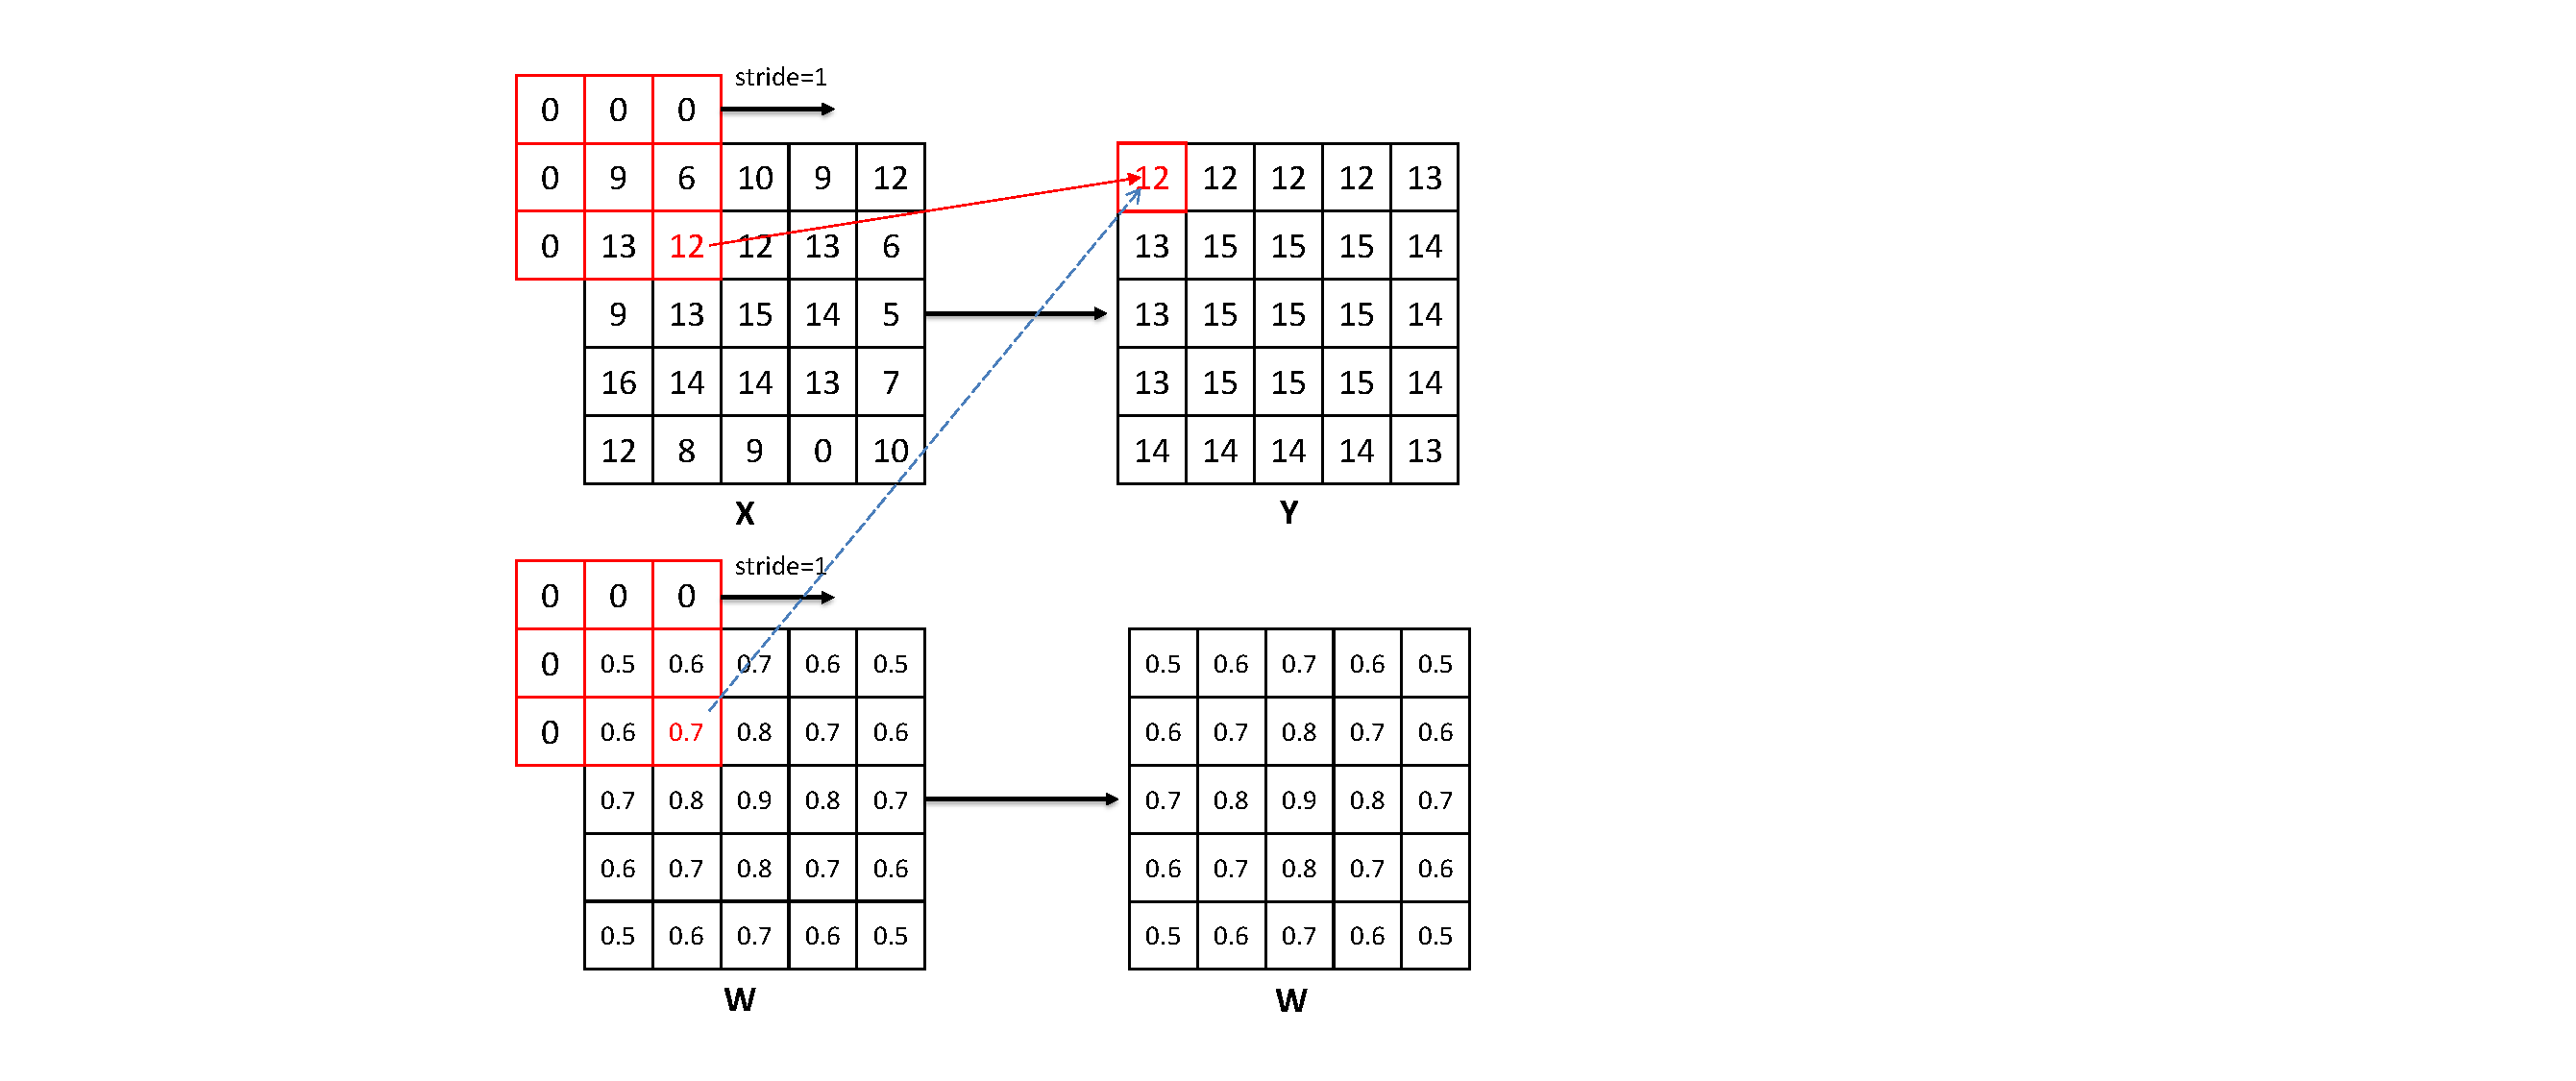
\includegraphics[width=3.4in]{figures/FigJMP.pdf}
   %\includegraphics[width=0.8\linewidth]{egfigure.eps}
    \end{center}
    \caption{An example of joint max pooling.
        Two windows of same size synchronously slide on $\mathbf{X}$ and $\mathbf{W}$.
       The elements in top window will be propagated the element under the indicator of bottom window.}
    \label{FigJMP}
\end{figure}

Based on this observation, we proposed a joint pooling layer \bobo{change a more accurate name?} by separating $\omega$ apart, rather than depend on $x$ or be fixed.
Explicitly, our joint pooling take two inputs, respectively denoted as $X$ and $W$ with same width and height.
During forward propagation, two windows with same size synchronously slide on $X$ and $W$, which are respectively denoted as $\mathcal{N}^{x}$ and $\mathcal{N}^{\omega}$.
Especially, $\mathcal{N}^{x}$ and $\mathcal{N}^{\omega}$ correspond to the same neighbor region $\mathcal{N}$ on different input maps.
The elements in $\mathcal{N}^{\omega}$ determine which elements in $\mathcal{N}^{x}$ will be propagated to next layer.
A simple example is illustrated in Figure~\ref{FigJMP}.

For max pooling, since $\omega_i$ is hard to be directly learned to be binary, a threshold function $\hbar(\cdot)$ is applied to $\omega_{i}$ by:
\begin{eqnarray}\label{jmp}
\begin{aligned}
y_{j} &= \sum_{i\in \mathcal{N}_{j}}x_{i}\hbar(\omega_{i},\mathcal{N}^{\omega}_{j})\\
\hbar(\omega_{i},\mathcal{N}^{\omega}_{j})&=\left\{\begin{array}{cc}
1&if~\omega_{i}\geq max(\mathcal{N}^{\omega}_{j})\\
0&else\\
\end{array}\right.
\end{aligned}
\end{eqnarray}
where $max(\cdot)$ finds the max value of the input.

It should be noted that in Figure~\ref{FigJMP} that elements $x_i$ in $X$ with small $\omega_i$ have been abandoned and substituted by $x_i$ with larger $\omega_i$ in $Y$.
If this processing is iterated more times, all the elements in $Y$ will be substituted by the $x_i$ with maximum $\omega_i$.
Back to our object segmentation task, it is reasonable to believe that objectness score $p_i$ in central region of an object are probably a local maximum point.
Therefore applying JMP to both outputs from multi-task FCN can well replace the predicted shape parameters in border area of an object with a nearest predictions in central area, which usually have local maximum $p_i$.
Explicitly, $p$, $t$ respectively corresponds to $W$, $X$, while $t$ is pooled under indication of $p$.
The pooling stride is fixed to be $1$ to maintain an unchanged resolution of final segmentation.
Pooling size and iteration times of JMP determine how far the $t_i$ with maximum $p_i$ can be spread.


Moreover, another contribution of our JMP is that the residual error can be correctly back propagated to its inputs.
This makes it a trainable layer in any network architecture and our SCNN become a fully trainable system.
Defining $L_{X}$ as the residual error on $X$ , the back propagation for $x_{i}$ can be expressed by:
\begin{eqnarray}\label{bpx}
\begin{aligned}
\frac{\partial L_\mathbf{X}}{\partial x_{i}}=\frac{1}{m}\sum\limits_{j\in\mathcal{N}_{i}}\frac{\partial L_{X}}{\partial y_{j}}\hbar(\omega_{i},{\mathcal{N}}^{\omega}_{j})\\
\end{aligned}
\end{eqnarray}
where $\mathcal{N}^{\omega}_{j}$ is the neighbor region centered on position $j$ in $W$ and $m$ is the size of $\mathcal{N}_{i}$.
Similar to forward propagation in original max pooling, Eq.~\ref{bpx} converge the gradients $\frac{\partial L_\mathbf{X}}{\partial y_{j}}$ into $x_{i}$ which has a local maximum $\omega_{i}$.
In this way, as most residual error $\frac{\partial L_\mathbf{X}}{\partial y_{j}}$ have been focused on area with high objectness scores by Eq.~\ref{bpx}, the predicted shape parameters in central area of objects will be more accurate.

%Specially in Figure \ref{FigSCNN}, the input segmentation map is assumed to not only influence the output but also feeds a subsequent layers, thus also receiving gradient contributions $\frac{\partial L}{\partial s_{i,j}}$ from the next layer during back-propagation.

Defining $L_{W}$ as the residual error on $W$.
It should be noted that our JMP will be iterated several times to spread $x_{i}$ with local maximum $\omega_{i}$ farther.
Therefore, we assume that $\omega_{i}$ not only influences the following $\{y_{j}|j\in\mathcal{N}_{i}\}$, but also receiving gradient contributions $\frac{\partial L_W}{\partial \omega_{i}}$ from subsequent JMP layer or shape supervised label during back-propagation.
The back propagation for $\omega_{i}$ is formulated by
%
\begin{eqnarray}\label{bps}
\begin{aligned}
\frac{\partial L_{W}}{\partial \omega_{i}}&=\frac{\partial L_{W}}{\partial \omega_{i}}+\frac{1}{m}\sum_{j\in\mathcal{N}_{i}}\frac{\partial L_{W}}{\partial y_{j}}\frac{\partial y_{j}}{\partial \omega_{i}}\\
&=\frac{\partial L_{W}}{\partial \omega_{i}}+\frac{1}{m}\sum_{j\in\mathcal{N}_{i}}\frac{\partial L_{W}}{\partial y_{j}}x_{i}\frac{\partial \hbar(\omega_{i},\mathcal{N}^{\omega}_{j})}{\partial \omega_{i}}\\
&=\frac{\partial L_{W}}{\partial \omega_{i}}+\frac{1}{m}\sum_{j\in\mathcal{N}_{i}}\frac{\partial L_{W}}{\partial y_{j}}x_{i}\delta(\omega_{i},\mathcal{N}^{\omega}_{j})\\
\end{aligned}
\end{eqnarray}
where $\delta(\omega_{i},\mathcal{N}^{\omega}_{j})$ is the derived function of $g(\omega_{i},\mathcal{N}^{\omega}_{j})$, which has an infinite response when $\omega_{i}$ is the maximum in $\mathcal{N}^{\omega}_{j}$.
In order to robustly propagate gradients to $\omega_{i}$, $\frac{\partial L_{W}}{\partial y_{j}}x_{i}$ is approximated by $\frac{\partial L_\mathbf{W}}{\partial \omega_{i}}$ multiplying a constant value $\alpha$  and $\delta(\omega_{i},\mathcal{N}^{\omega}_{j})$ is approximated to be $\hbar(\omega_{i},\mathcal{N}^{\omega}_{j})$.
Therefore, $\frac{\partial L_{W}}{\partial \omega_{i}}$ is formulated as a more concise form:
\begin{eqnarray}\label{dG}
\begin{aligned}
\frac{\partial L_{W}}{\partial \omega_{i}}&=\frac{\partial L_{W}}{\partial \omega_{i}}(1+\frac{1}{m}\sum_{j\in\mathcal{N}_{i}}\alpha \hbar(\omega_{i},\mathcal{N}^{\omega}_{j}))\\
\end{aligned}
\end{eqnarray}

Intuitively, Eq. \ref{dG} adds a loss weight on gradients of the local maximum $\omega_{i}$ with control of $\alpha$, which is beneficial to avoiding false and missing detection .

\subsection{Local Optimization for Final Segmentation}
\label{sec:fusion}
Based on the objectness map and auxiliary map of shape parameters obtained from joint max pooling, we now integrate the two types of information to produce more accurate boundaries.
Especially, the shape of objects in objectness map are predicted unrestrictedly by neural network without shape knowledge, while the shape of objects in auxiliary map are strictly constrained.
Therefore, it is important to reasonably fuse these two kinds of information into final segmentation mask.

In this section, a local optimization strategy is applied to allow our method to not only optimize the shape of regular objects, but also accommodate seriously deformable objects.
A key assumption in our local optimization strategy is that the shape of objects predicted in objectness map is approximate to the ground truth.
Hence we coarsely divide an objectness map into three parts: object area, contour area and background area.
The contour area is the ambiguous regions that is not sure to belong to object or background area.
In final segmentation mask, only the pixel in contour area are classified by predicted shape parameters, while the remaining pixels are classified by objectness scores.
For example with an objectness score $p_i$ and a set of parameters $t_i$ at position $i$, the classification result $m_i$ for pixel $i$ is determined by:
%
\begin{eqnarray}\label{fusion}
\begin{aligned}
m_i=\left\{\begin{array}{cc}
1&if~p_i>\tau_2\\
0&if~p_i<\tau_1\\
f(t_i)&else\\
\end{array}\right.
\end{aligned}
\end{eqnarray}
where $\tau_2$ and $\tau_1$ are two thresholds (set empirically) to control the degree of modification by prior shape constraint.
$f(t_i)$ is a function judging whether the pixel $i$ is within an object formulated by $t_i$.
As in our task an ellipse is defined by $ t_i = [\theta, \mu_c, \nu_c, a, b]$, the function is expressed by:
\begin{eqnarray}\label{fusion}
\begin{aligned}
f(t_i)&=\left\{\begin{array}{cc}
1&if~\frac{d\mu^2}{a^2}+\frac{d\nu^2}{b^2}<1\\
0&else\\
\end{array}\right.\\
dx &= cos(\theta)(\mu-\mu_c)+sin(\theta)(\nu-\nu_c)\\
dy &= -sin(\theta)(\mu-\mu_c)+cos(\theta)(\nu-\nu_c)\\
\end{aligned}
\end{eqnarray}
where $\mu$, $\nu$ are the spatial coordinates of pixel $i$. 

Our fusion strategy can appropriately utilize prior shape knowledge to not only separate touching objects into individual ones, but also optimize most regular object without losing generalization to deformable objects.
And our SCNN can be easily extended to other shape constraint, such as rectangle shape, circles by changing the form of shape parameters.
